\subsection{DNSSEC SNMP MIB implementation}
\label{section:dnssec-mib-implementation}
The OID entry point for the DNSSEC MIB is located inside the ARPA2 OID tree (enterprise OID 44469). The MIB module name is ARPA2-Experimental-DNSSEC-MIBv1 and is associated to the numerical OID \textit{.1.3.6.1.4.1.44469.666.53.46.161.1}. The path from the root down to that module is shown in Figure \ref{figure:oid-tree}

\begin{figure}[H]
\centering
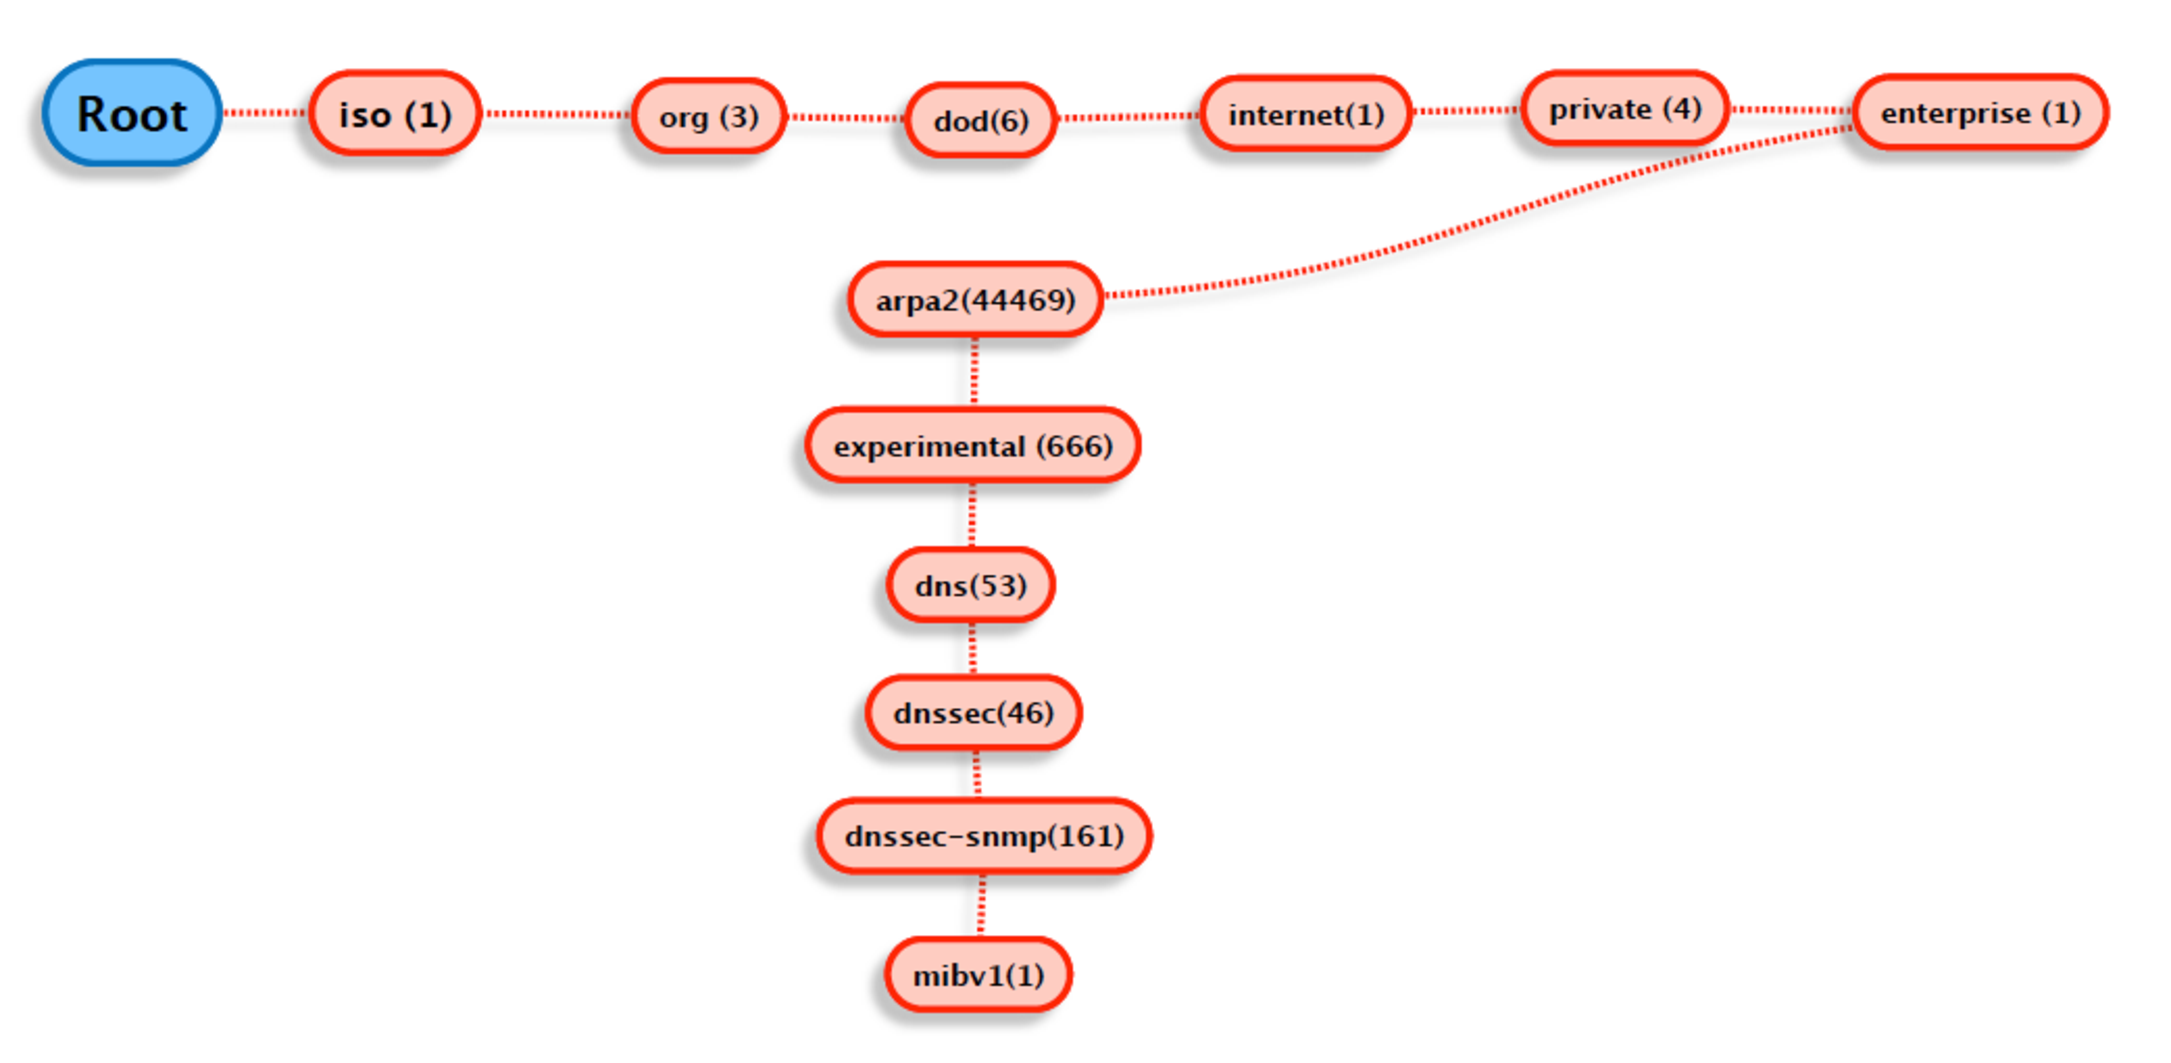
\includegraphics[scale=0.3]{Images/oid-tree.png}
\caption{OID Tree}
\label{figure:oid-tree}
\end{figure}


Objects defined in the MIB are organized as tables \footnote{in SNMP terminology tables are denoted as conceptual tables or columnar objects} or scalar types. Four tables which are indexed by domain name (OCTET-STRING) are included in the MIB (dnssecZoneGlobalTable, dnssecZoneAuthNSTable, dnssecZoneSigTable, dnssecZoneDiffTable). INTEGER datatypes are used to represent boolean and numeric values and data type  OCTET-STRING to represent strings (e.g domain names). Listing \ref{listing:snmptranslate} shows all top level elements of the created MIB including tables and their associated indexes.

\begin{listing}
\small\begin{verbatim}
+--arpa2experimentaldnssecMIBv1(1)
   |
   +--dnssecObjects(1)
   |  |
   |  +--dnssecGeneral(1)
   |  |  |
   |  +--dnssecZoneGlobal(2)
   |  |  |
   |  |  +--dnssecZoneGlobalTable(2)
   |  |     |
   |  |     +--dnssecZoneGlobalEntry(1)
   |  |        |  Index: dnssecZoneGlobalIndex
   |  |
   |  +--dnssecZoneAuthNS(3)
   |  |  |
   |  |  +--dnssecZoneAuthNSTable(3)
   |  |     |
   |  |     +--dnssecZoneAuthNSEntry(1)
   |  |        |  Index: dnssecZoneGlobalIndex
   |  |        |
   |  +--dnssecZoneSig(4)
   |  |  |
   |  |  +--dnssecZoneSigTable(4)
   |  |     |
   |  |     +--dnssecZoneSigEntry(1)
   |  |        |  Index: dnssecZoneGlobalIndex
   |  |        |
   |  +--dnssecZoneDiff(5)
   |     |
   |     +--dnssecZoneDiffTable(5)
   |        |
   |        +--dnssecZoneDiffEntry(1)
   |           |  Index: dnssecZoneGlobalIndex
   |           |
   +--dnssecMIBConformance(2)
      |
      +--dnssecMIBGroups(1)
      |  |
      |  +--dnssecMIBScalarGroup(1)
      |  +--dnssecMIBTableGroup(2)
      |
      +--dnssecMIBCompliances(2)

\end{verbatim}
\normalsize
\caption{Structure of ARPA2-Experimental-DNSSEC-MIBv1}
\label{listing:snmptranslate}
\end{listing}

To add more restrictions to the defined object-types and their indexes, textual conventions are used. Figure \ref{figure:textual-conventions} shows the impact of textual conventions for object-type \textit{dnssecZoneGlobalServFail} in table \textit{dnssecZoneGlobalTable}.    

\begin{figure}[H]
\centering
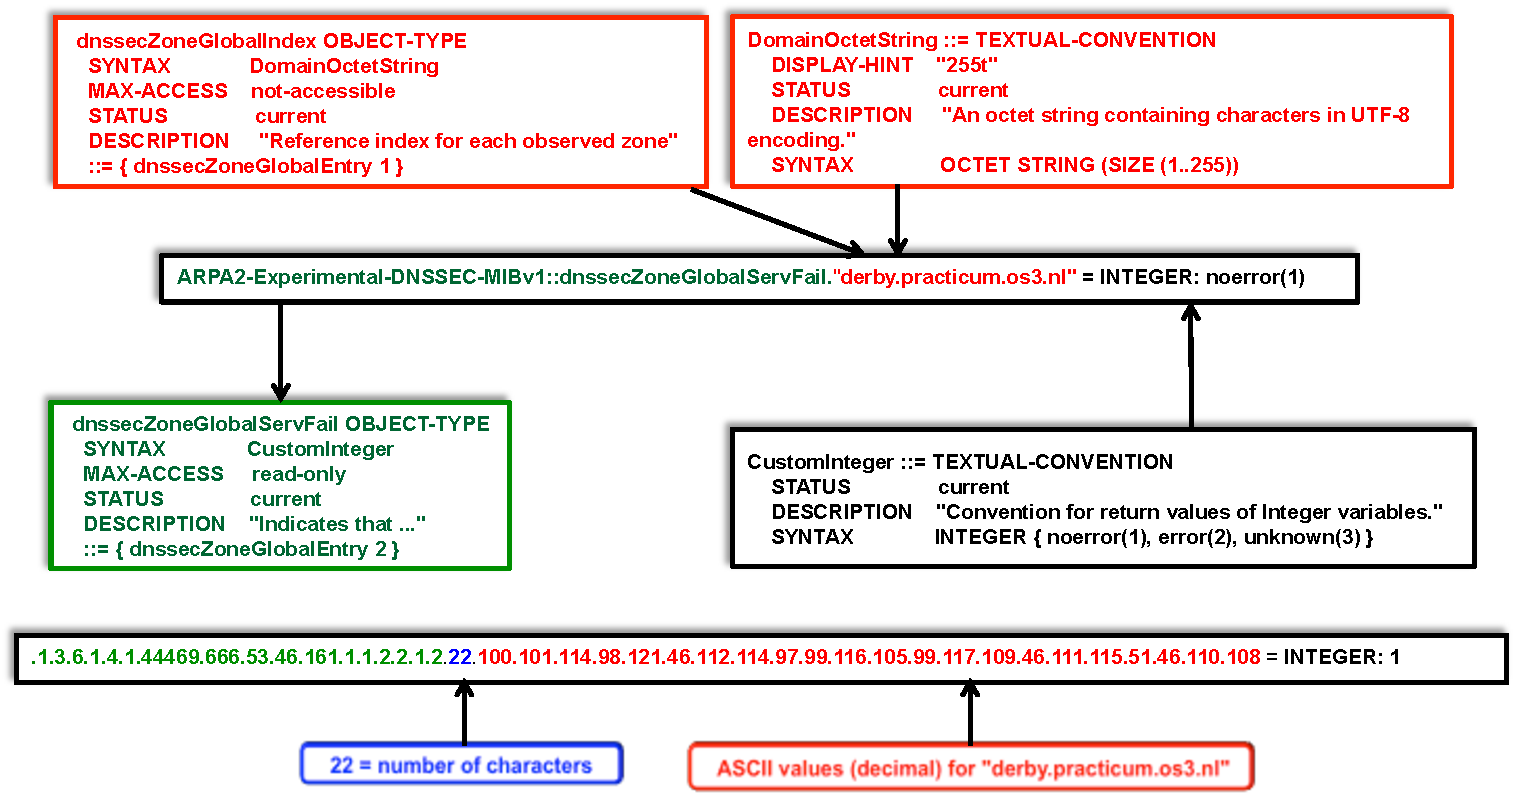
\includegraphics[scale=0.5]{Images/tc1.png}
\caption{Effect of textual conventions to represent MIB data}
\label{figure:textual-conventions}
\end{figure}

A textual convention \textit{DomainOctetString} is defined that is mapped to the \textit{dnssecZoneGlobalIndex}. That textual convention specifies the usage of the underlying datatype OCTET STRING and limits its number of octets to 255. That number represents the maximum allowed number of octets a domain name can contain \cite{wiki-domainnames}. Furthermore, the \textit{DISPLAY-HINT} clause specifies that characters of a string of that object-type will be UTF-8 encoded \cite{smi-tc}. That string, which represents a domain name is appended as an index value to each instance of an object-type.
\\ 
The textual convention \textit{CustomInteger} restricts the values that object-type \textit{dnssecZoneGlobalServFail} can have. In that case we allow the following values:

\begin{table}[h]
   \centering
  \begin{tabular}{|c|c|}
  \hline
  Value & Meaning \\
  \hline
  1 & No error \\
  2 & Error \\
  3 & Unknown \\  
  \hline
\end{tabular} 
\caption{Textual convention for integer variables }
\label{table}
\end{table}



That enables us to implement our agent data wrapper scripts in a way that for each check only these values can occur and we can associate them to a textual equivalent. 
\\
Figure \ref{figure:textual-conventions2} shows the numerical representation of an instance of object-type \textit{dnssecZoneGlobalServFail} and how the OID for the SNMP message is constructed.

\begin{figure}[H]
\centering
\includegraphics[scale=0.5]{Images/tc2.png}
\caption{numerical represenation of an instance of object-type dnssecZoneGlobalServFail}
\label{figure:textual-conventions2}
\end{figure}

The green marked numbers are the numerical identifiers for the object-type itself. Then the number of characters of the associated index is appended to the OID and finally the ASCII values in decimal for each character of the domain name.  